\documentclass[11pt]{article}

\usepackage{geometry}
 \geometry{
 a4paper,
 total={210mm,297mm},
 left=20mm,
 right=20mm,
 top=20mm,
 bottom=20mm,
 }
\usepackage{Sweave}
\usepackage{url}
\usepackage{rotating}
\usepackage{natbib}
\usepackage{placeins}
\usepackage{longtable}
\usepackage[latin1]{inputenc}
\usepackage{multirow}
\usepackage{hyperref}
%\usepackage{showframe}
\usepackage{pdflscape}
%\usepackage{pbox}

%\sloppy
%\SweaveOpts{echo=FALSE,prefix.string=script18/plot}
\renewcommand{\textfraction}{0.0}

\let\oldmarginpar\marginpar
\renewcommand\marginpar[1]{\-\oldmarginpar[\raggedleft\footnotesize #1]%
{\raggedright\footnotesize #1}}

\title{Introduction to RCSpin}
\author{Rob Dunne}
\date{\today}


\begin{document}
%\setkeys{Gin}{width=8cm}
\setkeys{Gin}{width=0.9\columnwidth}
\maketitle
\tableofcontents

\section{RCSpin}

This library implements the CRC-SPIN model \cite[]{Rutter.2008,Rutter.and.Savarino.2010}
using the Reference Classes object oriented system of R.  R how has 3 object systems, 
S3, S4, and Reference Classes (RC) systems.

RC is good for simulations with complex states.
It has mutable objects -- i.e changes don't make copies.
\marginpar{the class names are pointers, I think. Why is this a good idea? I don't know}





\section{genericSpin}
This class implements a natural aging model on a group of people
represented as a \texttt{study\_group} of \texttt{Person} class objects.
The main aim of this Class is to act as a framework for building more
complex models through extension of this class. The simple natural
aging model implemented in \texttt{updateSubject} acts as an
example and place holder for subclasses to override with a more
complex implementation of the function.

At the moment it subjects a population to the age specific mortality rates taken from a provided table.
See figure \ref{figure:GenericModel.png}.

The function \verb+help(GenericModel)+ provides help about the methods.
There is also  \verb+GenericModel(help)+ and
\verb+GenericModel$help(updateSubject)+ for help on specific methods.

 
 
\begin{Schunk}
\begin{Sinput}
> library(RCSpin)
> system.time(cc<-GenericModel(iterations=99, num_subjects=1000,base_seed=122))
> #   user  system elapsed 
> # 10.473   0.016  10.631 
> 
> system.time(cc$run())
> #140.140   0.084 140.779 
> 
> 
> plot(1:99,res.M,col="blue",ylim=c(0,550),type="n",
+      xlab="age",ylab="population")
> temp<-rep(0,99)
> temp[1]<-number.M
> for ( ii in 2:99){
+     temp[ii]<- temp[ii-1]-death_rate_male[ii-1]*temp[ii-1]
+ }
> lines(temp,col="blue")
> temp<-rep(0,99)
> temp[1]<-number.F
> for ( ii in 2:99){
+     temp[ii]<- temp[ii-1]-death_rate_female[ii-1]*temp[ii-1]
+ }
> lines(temp,col="red")
> legend(20,300,c("male","female"),col=c("blue","red"),lty=1)
\end{Sinput}
\end{Schunk}

\begin{figure}[tbhp]
  \centering
  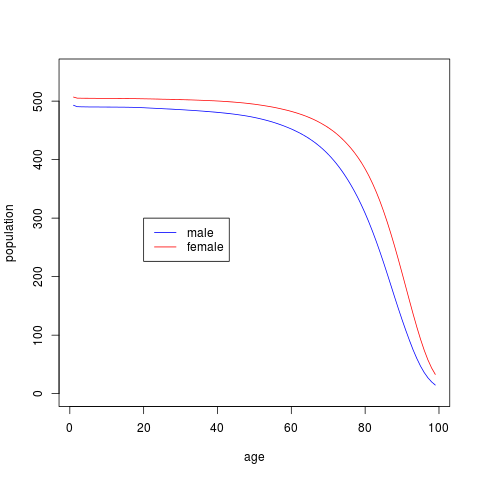
\includegraphics[totalheight=9cm]{./figs/GenericModel.png}
  \caption{A population of 1000 peoiple subjected to the mortality rates of a supplied table.}
  \label{figure:GenericModel.png}
\end{figure}

\FloatBarrier
\section{crcSpin}

\begin{Schunk}
\begin{Sinput}
> #ccsm<-CrcSpinModel$new(iterations=99, num_subjects=50000,base_seed=122)
> #ccsm$run()
> #dim(ccsm$study_results)# 198  18
> #CrcSpinModel_output<- organize_results(ccsm)
> 
> data(CrcSpinModel_output)
> attach(CrcSpinModel_output)
> plot(results.M$colon.state.large.adenoma/number.M,type="l",col="orange",lwd=2,
+      xlab="age",axes=FALSE,
+      ylab="proportion of population",ylim=c(0,0.1),
+           main="CRC -- male population with no screening")
> lines(results.M$colon.state.pre.symptomatic.CRC/number.M,col="plum4",lwd=2)
> lines(results.M$colon.state.CRC/number.M,col="purple",lwd=2)
> legend(20,0.07,c("population","large adenoma", "CRC","symptomatic CRC"), 
+        col=c("green","orange","plum4","purple"),lwd=2)
> axis(2, pretty( c(0,0.1),10))
> par(new=TRUE)
> plot(pp<- number.M-cumsum(results.M$person.state.deceased),axes=FALSE,type="l",
+      ylab="",xlab="",lty=1,col=3,lwd=2 )
> axis(4, pretty(range(c(0,number.M),10)))
> mtext(side=4, line=3, "population")
> axis(1,pretty(range(1:99),10))
> box() #- to make it look "as usual"
> 
\end{Sinput}
\end{Schunk}

\begin{figure}[tbhp]
  \centering
  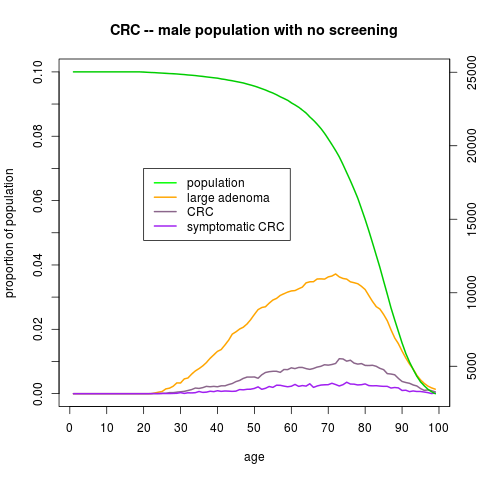
\includegraphics[totalheight=9cm]{./figs/CrcSpinModel.png}
  \caption{A population of 5000 peoiple subjected to the CRC-SPIN model.}
  \label{figure:CrcSpinModel.png}
\end{figure}

\FloatBarrier
\section{DukesCrcSpinModel}


\begin{Schunk}
\begin{Sinput}
> #dddm<-DukesCrcSpinModel$new(iterations=99, num_subjects=50000, base_seed=125, 
> #   commencement_age=20)
> #dddm$run()
> #dim(dddm$study_results)  #198  60
> #aa<-organize_results(dddm)
> 
> data(DukesCrcSpinModel_output)
> attach(DukesCrcSpinModel_output)
> plot(results.M$colon.state.large.adenoma/number.M,type="l",col="orange",lwd=2,
+      xlab="age",axes=FALSE, ylab="proportion of population",ylim=c(0,0.1),
+           main="CRC -- male population with no screening")
> lines(results.M$colon.state.CRC/number.M,col="plum4",lwd=2)
> lines(results.M$colon.state.symptomatic.CRC/number.M,col="purple",lwd=2)
> legend(20,0.07,c("population","large adenoma", "CRC","symptomatic CRC"), 
+        col=c("green","orange","plum4","purple"),lwd=2)
> axis(2, pretty( c(0,0.1),10))
> par(new=TRUE)
> plot(pp<- number.M-cumsum(results.M$person.state.deceased),axes=FALSE,
+       type="l",ylab="",xlab="",lty=1,col=3,lwd=2 )
> axis(4, pretty(range(c(0,number.M),10)))
> mtext(side=4, line=3, "population")
> axis(1,pretty(range(1:99),10))
> box() #- to make it look "as usual"
> y<-results.M[,40:44]  #person1@colon@stage  includes CRC and pre-symptomatic     
> x<-c(1:99)
> z<-c(1,2,3,4,5) #z <- val2col(apply(y,2,max), col=COLS)
> #ylim=c(0, 1.2*max(apply(y,1,sum), na.rm=TRUE))
> 
> #png("t7.png")
> par(mfrow=c(3,1))
> plot.stacked(x,y, xlim=c(0, 100), ylim=c(0, 500),
+               yaxs="i", col=z, border="white", lwd=0.5,order.method="as.is")
> title(main="all CRC, population of 25000 males")
> y<-res.M[,54:57]     #   found from test or symptoms      
> z<-c(1,2,3,4) 
> plot.stacked(x,y, xlim=c(0, 100),  ylim=c(0, 500),
+               yaxs="i", col=z, border="white", lwd=0.5,order.method="as.is")
> title(main="entering treatment -- detected by NBCSP")
> y<-res.M[,12:16]     #                        if (object@colon@state=="pre symptomatic CRC"){
> z<-c(1,2,3,4,5)
> plot.stacked(x,y, xlim=c(0, 100), ylim=c(0, 500),
+               yaxs="i", col=z, border="white", lwd=0.5,order.method="as.is")
> title(main="undetected  CRC")
> #dev.off()
> abline(v=c(55,60,65,70,75))
> ###############################################################################
> ## http://www.r-bloggers.com/data-mountains-and-streams-stacked-area-plots-in-r/
> ##plot.stacked makes a stacked plot where each y series is plotted on top
> ##of the each other using filled polygons
> ##
> ##Arguments include:
> ## 'x' - a vector of values
> ## 'y' - a matrix of data series (columns) corresponding to x
> ## 'order.method' = c("as.is", "max", "first")
> ## "as.is" - plot in order of y column
> ## "max" - plot in order of when each y series reaches maximum value
> ## "first" - plot in order of when each y series first value > 0
> ## 'col' - fill colors for polygons corresponding to y columns (will recycle)
> ## 'border' - border colors for polygons corresponding to y columns (will recycle) (see ?polygon for details)
> ## 'lwd' - border line width for polygons corresponding to y columns (will recycle)
> ## '...' - other plot arguments
> 
> plot.stacked <- function(x, y,order.method = "as.is",ylab="", xlab="",
+                          border = NULL, lwd=1,
+                          col=rainbow(length(y[1,])),
+                          ylim=NULL,
+                          ...
+                          ){
+     
+     if(sum(y < 0) > 0) error("y cannot contain negative numbers")
+     
+     if(is.null(border)) border <- par("fg")
+     border <- as.vector(matrix(border, nrow=ncol(y), ncol=1))
+     col <- as.vector(matrix(col, nrow=ncol(y), ncol=1))
+     lwd <- as.vector(matrix(lwd, nrow=ncol(y), ncol=1))
+     
+     if(order.method == "max") {
+         ord <- order(apply(y, 2, which.max))
+         y <- y[, ord]
+         col <- col[ord]
+         border <- border[ord]
+     }
+     
+     if(order.method == "first") {
+         ord <- order(apply(y, 2, function(x) min(which(r>0))))
+         
+         
+         y <- y[, ord]
+         col <- col[ord]
+         border <- border[ord]
+     }
+     
+     top.old <- x*0
+     polys <- vector(mode="list", ncol(y))
+     for(i in seq(polys)){
+         top.new <- top.old + y[,i]
+         polys[[i]] <- list(x=c(x, rev(x)), y=c(top.old, rev(top.new)))
+         top.old <- top.new
+     }
+     
+     if(is.null(ylim)) ylim <- range(sapply(polys, function(x) range(x$y, na.rm=TRUE)), na.rm=TRUE)
+     plot(x,y[,1], ylab=ylab, xlab=xlab, ylim=ylim, t="n", ...)
+     for(i in seq(polys)){
+         polygon(polys[[i]], border=border[i], col=col[i], lwd=lwd[i])
+     }
+     
+ }
> #plot.stream makes a "stream plot" where each y series is plotted
> #as stacked filled polygons on alternating sides of a baseline.
> #
> #Arguments include:
> #'x' - a vector of values
> #'y' - a matrix of data series (columns) corresponding to x
> #'order.method' = c("as.is", "max", "first")
> # "as.is" - plot in order of y column
> # "max" - plot in order of when each y series reaches maximum value
> # "first" - plot in order of when each y series first value > 0
> #'center' - if TRUE, the stacked polygons will be centered so that the middle,
> #i.e. baseline ("g0"), of the stream is approximately equal to zero.
> #Centering is done before the addition of random wiggle to the baseline.
> #'frac.rand' - fraction of the overall data "stream" range used to define the range of
> #random wiggle (uniform distrubution) to be added to the baseline 'g0'
> #'spar' - setting for smooth.spline function to make a smoothed version of baseline "g0"
> #'col' - fill colors for polygons corresponding to y columns (will recycle)
> #'border' - border colors for polygons corresponding to y columns (will recycle) (see ?polygon for details)
> #'lwd' - border line width for polygons corresponding to y columns (will recycle)
> #'...' - other plot arguments
>  
> plot.stream <- function( x, y, order.method = "as.is", frac.rand=0.1,
+                         spar=0.2, center=TRUE, ylab="", xlab="", border = NULL, lwd=1,
+                         col=rainbow(length(y[1,])), ylim=NULL, ...  ){
+     
+     if(sum(y < 0) > 0) error("y cannot contain negative numbers")
+     
+     if(is.null(border)) border <- par("fg")
+     border <- as.vector(matrix(border, nrow=ncol(y), ncol=1))
+     col <- as.vector(matrix(col, nrow=ncol(y), ncol=1))
+     lwd <- as.vector(matrix(lwd, nrow=ncol(y), ncol=1))
+     
+     if(order.method == "max") {
+         ord <- order(apply(y, 2, which.max))
+         y <- y[, ord]
+         col <- col[ord]
+         border <- border[ord]
+     }
+     
+     if(order.method == "first") {
+ 	ord <- order(apply(y, 2, function(x) min(which(r>0))))
+         y <- y[, ord]
+         col <- col[ord]
+         border <- border[ord]
+     }
+     
+     bottom.old <- x*0
+     top.old <- x*0
+     polys <- vector(mode="list", ncol(y))
+     for(i in seq(polys)){
+         if(i %% 2 == 1){ #if odd
+             top.new <- top.old + y[,i]
+             polys[[i]] <- list(x=c(x, rev(x)), y=c(top.old, rev(top.new)))
+             top.old <- top.new
+         }
+         if(i %% 2 == 0){ #if even
+             bottom.new <- bottom.old - y[,i]
+             polys[[i]] <- list(x=c(x, rev(x)), y=c(bottom.old, rev(bottom.new)))
+             bottom.old <- bottom.new
+         }
+ }
+  
+     ylim.tmp <- range(sapply(polys, function(x) range(x$y, na.rm=TRUE)), na.rm=TRUE)
+     outer.lims <- sapply(polys, function(r) rev(r$y[(length(r$y)/2+1):length(r$y)]))
+     mid <- apply(outer.lims, 1, function(r) mean(c(max(r, na.rm=TRUE), min(r, na.rm=TRUE)), na.rm=TRUE))
+                                         #center and wiggle
+     if(center) {
+         g0 <- -mid + runif(length(x), min=frac.rand*ylim.tmp[1], max=frac.rand*ylim.tmp[2])
+     } else {
+         g0 <- runif(length(x), min=frac.rand*ylim.tmp[1], max=frac.rand*ylim.tmp[2])
+     }
+     fit <- smooth.spline(g0 ~ x, spar=spar)
+     
+     for(i in seq(polys)){
+         polys[[i]]$y <- polys[[i]]$y + c(fit$y, rev(fit$y))
+     }
+     
+     if(is.null(ylim)) ylim <- range(sapply(polys, function(x) range(x$y, na.rm=TRUE)), na.rm=TRUE)
+     plot(x,y[,1], ylab=ylab, xlab=xlab, ylim=ylim, t="n", ...)
+     for(i in seq(polys)){
+         polygon(polys[[i]], border=border[i], col=col[i], lwd=lwd[i])
+     }
+     
+ }
> #this function converts a vector of values("z") to a vector of color
> #levels. One must define the number of colors. The limits of the color
> #scale("zlim") or the break points for the color changes("breaks") can 
> #also be defined. when breaks and zlim are defined, breaks overrides zlim.
> val2col<-function(z, zlim, col = heat.colors(12), breaks){
+     if(!missing(breaks)){
+         if(length(breaks) != (length(col)+1)){stop("must have one more break than colour")}
+     }
+     if(missing(breaks) & !missing(zlim)){
+         zlim[2] <- zlim[2]+c(zlim[2]-zlim[1])*(1E-3)#adds a bit to the range in both directions
+         zlim[1] <- zlim[1]-c(zlim[2]-zlim[1])*(1E-3)
+         breaks <- seq(zlim[1], zlim[2], length.out=(length(col)+1)) 
+     }
+     if(missing(breaks) & missing(zlim)){
+         zlim <- range(z, na.rm=TRUE)
+         zlim[2] <- zlim[2]+c(zlim[2]-zlim[1])*(1E-3)#adds a bit to the range in both directions
+         zlim[1] <- zlim[1]-c(zlim[2]-zlim[1])*(1E-3)
+         breaks <- seq(zlim[1], zlim[2], length.out=(length(col)+1))
+     }
+     CUT <- cut(z, breaks=breaks)
+     colorlevels <- col[match(CUT, levels(CUT))] # assign colors to heights for each point
+     return(colorlevels)
+ }
> 
> 
> ## set.seed(1)
> ## m <- 500
> ## n <- 30
> ## x <- seq(m)
> ## y <- matrix(0, nrow=m, ncol=n)
> ## colnames(y) <- seq(n)
> ## for(i in seq(ncol(y))){
> ## mu <- runif(1, min=0.25*m, max=0.75*m)
> ## SD <- runif(1, min=5, max=20)
> ## TMP <- rnorm(1000, mean=mu, sd=SD)
> ## HIST <- hist(TMP, breaks=c(0,x), plot=FALSE)
> ## fit <- smooth.spline(HIST$counts ~ HIST$mids)
> ## y[,i] <- fit$y
> ## }
> ## y <- replace(y, y<0.01, 0)
>  
>  
> ## #Plot Ex. 1 - Color by max value
> ## pal <- colorRampPalette(c(rgb(0.85,0.85,1), rgb(0.2,0.2,0.7)))
> ## BREAKS <- pretty(apply(y,2,max),8)
> ## LEVS <- levels(cut(1, breaks=BREAKS))
> ## COLS <- pal(length(BREAKS )-1)
> ## z <- val2col(apply(y,2,max), col=COLS)
>  
> ## #plot.stacked(x,y, xlim=c(100, 400), ylim=c(0, 1.2*max(apply(y,1,sum), na.rm=TRUE)),
> ## #             yaxs="i", col=z, border="white", lwd=0.5)
> 
> 
> 
\end{Sinput}
\end{Schunk}



\begin{figure}[tbhp]
  \centering
  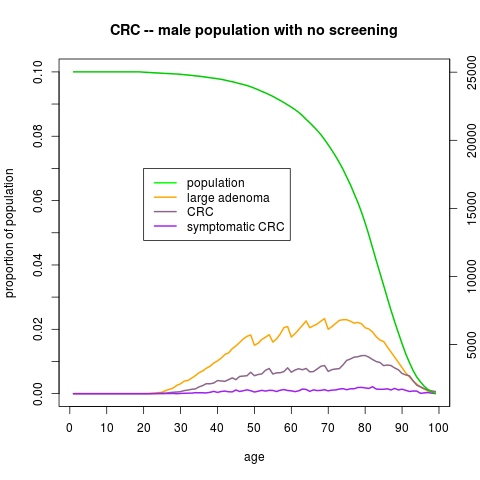
\includegraphics[totalheight=9cm]{./figs/DukesCrcSpinModel.png}
  \caption{A population of 5000 peoiple subjected to the CRC-SPIN model.}
  \label{figure:DukesCrcSpinModel.png}
\end{figure}


\clearpage
\begin{thebibliography}{}

%\bibliographystyle{apalike}
%\bibliography{RCSpin}
%% M-n P to create a tex file then bibtex to create the .bbl file
%% then include the .bbl file here
  
\bibitem[Rutter, 2008]{Rutter.2008}
Rutter, C. (2008).
\newblock Group health research institute ({CRC-SPIN}).
\newblock Version: HI.001.10242008.41523. Document generated: 10/24/2008
  \url{https://cisnet.flexkb.net/mp/pub/cisnet_colorectal_ghc_profile.pdf}.

\bibitem[Rutter and Savarino, 2010]{Rutter.and.Savarino.2010}
Rutter, C.~M. and Savarino, J.~E. (2010).
\newblock An evidence-based microsimulation model for colorectal cancer:
  validation and application.
\newblock {\em Cancer Epidemiol Biomarkers Prev}, 19(8):1992--2002.
\newblock Epub 2010 Jul 20.
\end{thebibliography}


\appendix
\section{outputs}
%% \begin{sidewaystable}[htbp]
%%   \centering
%%   \begin{tabular}[h]{||l|p{20cm}||}
%% \hline
%%  1  &    count(adenoma.state=="adenoma");        A count of adenomas in all patients of the study group that have state "adenoma"    \\
%%  2  &    count(adenoma.state=="large adenoma");  A count of adenomas in all patients of the study group that have state "large adenoma" \\
%%  3  &    count(adenoma.state=="pre symptomatic CRC");    A count of adenomas in all patients of the study group that have state "pre symptomatic CRC" \\
%%  4  &    count(person.colon\_clinical=="CRC");    A count of patients that have colon\_clinical state "CRC" \\
%%  5  &    count(colon.state=="clear");    A count of how many peoples colons were in state "clear" \\
%%  6  &    count(colon.state=="adenoma");  A count of how many peoples colons were in state "adenoma" \\
%%  7  &    count(colon.state=="large adenoma");    A count of how many peoples colons were in state "large adenoma" \\
%%  8  &    count(colon.state=="pre symptomatic CRC");      A count of how many peoples colons were in state "pre symptomatic CRC" \\
%%  9  &    count(colon.state=="CRC");      A count of how many peoples colons were in state "CRC" \\
%%  10 &    count(colon.cancer\_site=="cecum");      A count of how many people's colons overall that have the majority of their adenomas in the "cecum" location \\
%%  11 &    count(colon.cancer\_site=="ascending");  A count of how many people's colons overall that have the majority of their adenomas in the "ascending" location \\
%%  12 &    count(colon.cancer\_site=="transverse");         A count of how many people's colons overall that have the majority of their adenomas in the "transverse" location \\
%%  13 &    count(colon.cancer\_site=="descending");         A count of how many people's colons overall that have the majority of their adenomas in the "descending" location \\
%%  14 &    count(colon.cancer\_site=="sigmoid");    A count of how many people's colons overall that have the majority of their adenomas in the "sigmoid" location \\
%%  15 &    count(colon.cancer\_site=="rectum");     A count of how many people's colons overall that have the majority of their adenomas in the "rectum" location \\
%%  16 &    count(person.state=="deceased");        A count of people in the study that have died (i.e. their state is "deceased") \\
%%  17 &    count(person.colon\_clinical=="CRC");    A count of patients that have colon\_clinical state "CRC" \\
%%  18 &    count(where(person.initiateCRCTreatment() called))  // => person.in\_treatment\_program   A count of people put into a treatment program THIS ITERATION!!! \\
%% \hline
%%   \end{tabular}
%%   \caption{summary of genes in common in ``Top 200'', pairwise comparisons}
%%   \label{table:summary}
%% \end{sidewaystable}

%M-x <RET> toggle-truncate-lines <RET>
%Alternatively, you can set the default value for all buffers for the duration of a session with the following command:
%M-x <RET> set-variable <RET> truncate-lines <RET> t


\begin{landscape}
%%   \sloppy
%% \tolerance 1414
%% \hbadness 1414
%% \emergencystretch 1.5em
%% \hfuzz 0.3pt
%% \widowpenalty=10000
%% \vfuzz \hfuzz
%% \raggedbottom
  \raggedright
%\begin{longtable}{||l|l|p{12cm}|p{10cm}||}
\begin{longtable}{||l|l|p{11.3cm}|p{11.3cm}||}
\hline
\rotatebox{80}{DukesCrcSpin} & \rotatebox{80}{CrcSpin} & Expression                                                                    & Description  \\
\hline \\
1            & 1       & count(adenoma.state=="adenoma");                                              & A count of adenomas in all patients of the study group that have state "adenoma" \\
2            & 2       & count(adenoma.state=="large adenoma");                                        & A count of adenomas in all patients of the study group that have state "large adenoma" \\
3            & 3       & count(adenoma.state=="CRC");                                                  & A count of adenomas in all patients of the study group that have state "CRC" \\
4            & .       & count(adenoma.state=="deceased");                                             & A count of adenomas in all patients of the study group that have state "deceased" \\
5            & 4       & count(person.colon\_clinical=="symptomatic CRC");                              & A count of patients that have colon\_clinical state "symptomatic CRC" \\
6            & 5       & count(colon.state=="clear");                                                  & A count of how many peoples colons were in state "clear" \\
7            & 6       & count(colon.state=="adenoma");                                                & A count of how many peoples colons were in state "adenoma" \\
8            & 7       & count(colon.state=="large adenoma");                                          & A count of how many peoples colons were in state "large adenoma" \\
9            & 8       & count(colon.state=="CRC");                                                    & A count of how many peoples colons were in state "CRC" \\
10           & 9       & count(colon.state=="symptomatic CRC");                                        & A count of how many peoples colons were in state "symptomatic CRC" \\
11           & .       & count(colon.state=="deceased");                                               & A count of how many peoples colons were in state "deceased" \\
12           & .       & count(colon.state=="CRC" \&\& adenoma.stage=="A");                            &   A count of the adenomas that are at stage "A" in colons with state "CRC" across all people in the study group \\
13           & .       & count(colon.state=="CRC" \&\& adenoma.stage=="B");                            &   A count of the adenomas that are at stage "B" in colons with state "CRC" across all people in the study group \\
14           & .       & count(colon.state=="CRC" \&\& adenoma.stage=="C");                            &   A count of the adenomas that are at stage "C" in colons with state "CRC" across all people in the study group \\
15           & .       & count(colon.state=="CRC" \&\& adenoma.stage=="D");                            &   A count of the adenomas that are at stage "D" in colons with state "CRC" across all people in the study group \\
16           & .       & count(colon.state=="CRC" and adenoma.stage=="deceased");                      &   A count of the adenomas that are at stage "deceased" in colons with state "CRC" in all people in the study group \\
17           & .       & count(colon.state=="CRC" \&\& colon.cancer\_site=="cecum");                    &   A count of colons in "state" that have the majority of their adenomas in the "cecum" location across all people in the study group \\
18           & .       & count(colon.state=="CRC" \&\& colon.cancer\_site=="ascending");                &   A count of colons in "state" that have the majority of their adenomas in the "ascending" location across all people in the study group \\
19           & .       & count(colon.state=="CRC" \&\& colon.cancer\_site=="transverse");               &   A count of colons in "state" that have the majority of their adenomas in the "transverse" location across all people in the study group \\
20           & .       & count(colon.state=="CRC" \&\& colon.cancer\_site=="descending");               &   A count of colons in "state" that have the majority of their adenomas in the "descending" location across all people in the study group \\
21           & .       & count(colon.state=="CRC" \&\& colon.cancer\_site=="sigmoid");                  &   A count of colons in "state" that have the majority of their adenomas in the "sigmoid" location across all people in the study group \\
22           & .       & count(colon.state=="CRC" \&\& colon.cancer\_site=="rectum");                   &   A count of colons in "state" that have the majority of their adenomas in the "rectum" location across all people in the study group \\
23           & .       & count(colon.state=="symptomatic CRC" \&\& adenoma.stage=="A");                &   A count of the adenomas that are at stage "A" in people of the study group with colon\_clinical set to "symptomatic CRC" \\
24           & .       & count(colon.state=="symptomatic CRC" \&\& adenoma.stage=="B");                &   A count of the adenomas that are at stage "B" in people of the study group with colon\_clinical set to "symptomatic CRC" \\
25           & .       & count(colon.state=="symptomatic CRC" \&\& adenoma.stage=="C");                &   A count of the adenomas that are at stage "C" in people of the study group with colon\_clinical set to "symptomatic CRC" \\
26           & .       & count(colon.state=="symptomatic CRC" \&\& adenoma.stage=="D");                &   A count of the adenomas that are at stage "D" in people of the study group with colon\_clinical set to "symptomatic CRC" \\
27           & .       &  count(colon.state=="symptomatic CRC" \&\& adenoma.stage=="deceased");         &   A count of the adenomas that are at stage "deceased" in people of the study group with colon\_clinical set to "symptomatic CRC" \\
27           & .       & \centering{ count(colon.state=="symptomatic CRC" \&\& adenoma.stage=="deceased");    }     &   A count of the adenomas that are at stage "deceased" in people of the study group with colon\_clinical set to "symptomatic CRC" \\
28           & .       & count(colon.state=="symptomatic CRC" \&\& colon.cancer\_site=="cecum");        &   A count of colons in "state" that have the majority of their adenomas in the "cecum" location across all people in the study group \\
29           & .       & count(colon.state=="symptomatic CRC" \&\& colon.cancer\_site=="ascending");    &   A count of colons in "state" that have the majority of their adenomas in the "ascending" location across all people in the study group \\
30           & .       & count(colon.state=="symptomatic CRC" \&\& colon.cancer\_site=="transverse");   &   A count of colons in "state" that have the majority of their adenomas in the "transverse" location across all people in the study group \\
31           & .       & count(colon.state=="symptomatic CRC" \&\& colon.cancer\_site=="descending");   &   A count of colons in "state" that have the majority of their adenomas in the "descending" location across all people in the study group \\
32           & .       & count(colon.state=="symptomatic CRC" \&\& colon.cancer\_site=="sigmoid");      &   A count of colons in "state" that have the majority of their adenomas in the "sigmoid" location across all people in the study group \\
33           & .       & count(colon.state=="symptomatic CRC" \&\& colon.cancer\_site=="rectum");       &   A count of colons in "state" that have the majority of their adenomas in the "rectum" location across all people in the study group \\
34           & 10      & count(colon.cancer\_site=="cecum");                                            & A count of how many people's colons overall that have the majority of their adenomas in the "cecum" location \\
35           & 11      & count(colon.cancer\_site=="ascending");                                        & A count of how many people's colons overall that have the majority of their adenomas in the "ascending" location \\
36           & 12      & count(colon.cancer\_site=="transverse");                                       & A count of how many people's colons overall that have the majority of their adenomas in the "transverse" location \\
37           & 13      & count(colon.cancer\_site=="descending");                                       & A count of how many people's colons overall that have the majority of their adenomas in the "descending" location \\
38           & 14      & count(colon.cancer\_site=="sigmoid");                                          & A count of how many people's colons overall that have the majority of their adenomas in the "sigmoid" location \\
39           & 15      & count(colon.cancer\_site=="rectum");                                           & A count of how many people's colons overall that have the majority of their adenomas in the "rectum" location \\
40           & .       & count(colon.stage=="A");                                                      & A count of how many people's colons overall were in stage "A" \\
41           & .       & count(colon.stage=="B");                                                      & A count of how many people's colons overall were in stage "B" \\
42           & .       & count(colon.stage=="C");                                                      & A count of how many people's colons overall were in stage "C" \\
43           & .       & count(colon.stage=="D");                                                      & A count of how many people's colons overall were in stage "D" \\
44           & .       & count(colon.stage=="deceased");                                               & A count of how many people's colons overall were in stage "deceased" \\
.            & 16      & count(person.state=="deceased");                                              & A count of people in the study that have died (i.e. their state is "deceased") \\
45           & .       & count(person.state=="deceased" || person.state=="deceased CRC");              & A count of people in the study that have died (i.e. their state is "deceased" or "deceased CRC") \\
46           & 17      & count(person.colon\_clinical=="symptomatic CRC");                              & A count of patients that have colon\_clinical state "symptomatic CRC" \\
47           & .       & FALSE|0 (not implemented)                                                     & \\
48           & .       & FALSE|0 (not implemented)                                                     & \\
49           & .       & FALSE|0 (not implemented)                                                     & \\
50           & .       & FALSE|0 (not implemented)                                                     & \\
51           & .       & FALSE|0 (not implemented)                                                     & \\
52           & .       & count(where( person.initiateCRCTreatment() called)  \&\& (colonoscopy\_performed))  & A count of people that where treated for CRC IN THIS ITERATION, in which a colonoscopy was performed \\
53           & .       & count(where(person.initiateCRCTreatment() called)    \&\&(colon.state=="adenoma" || colon.state=="large adenoma"))                            & A count of people that where treated for CRC IN THIS ITERATION, who had colons in state "adenoma" or "large adenoma" \\
54           & .       & count(where(person.initiateCRCTreatment() called)   \&\&(colon.state=="symptomatic CRC" \&\& colon.stage=="A"))                            & A count of people that where treated for CRC IN THIS ITERATION, who had colons in state "symptomatic CRC" and in stage "A" \\
55           & .       & count(where(person.initiateCRCTreatment() called)             \&\&(colon.state=="symptomatic CRC" \&\& colon.stage=="B"))                        & A count of people that where treated for CRC IN THIS ITERATION, who had colons in state "symptomatic CRC" and in stage "B" \\
56           & .       & count(where(person.initiateCRCTreatment() called)                \&\&(colon.state=="symptomatic CRC" \&\& colon.stage=="C"))                 & A count of people that where treated for CRC IN THIS ITERATION, who had colons in state "symptomatic CRC" and in stage "C" \\
57           & .       & count(where(person.initiateCRCTreatment() called)       \&\&(colon.state=="symptomatic CRC" \&\& colon.stage=="D"))                          & A count of people that where treated for CRC IN THIS ITERATION, who had colons in state "symptomatic CRC" and in stage "D" \\
58           & 18      & count(where(person.initiateCRCTreatment() called))   // => person.in\_treatment\_program                               & A count of people put into a treatment program THIS ITERATION!!! \\
59           & .       & count(where(person.initiateCRCTreatment() called)    \&\& colonoscopy\_performed \&\& colonoscopy\_caused\_bleeding)                              & A count of people that where treated for CRC IN THIS ITERATION, whose colonoscopy caused bleeding \\
60           & .       & count(where(person.initiateCRCTreatment() called)   \&\& colonoscopy\_performed \&\& colonoscopy\_caused\_perforation)                              & A count of people that where treated for CRC IN THIS ITERATION, whose colonoscopy caused perforation \\
\hline
%  \end{tabular}
  \caption{summary of genes in common in ``Top 200'', pairwise comparisons}
  \label{table:summary}
\end{longtable}
\end{landscape}


%% \begin{landscape}
%% \begin{longtable}{||l|l|p{15cm}|p{10cm}||}
%% %  \centering
%% %  \begin{tabular}[h]{||l|l|p{16cm}|p{8cm}||}
%% \hline
%% \rotatebox{80}{DukesCrcSpin} & \rotatebox{80}{CrcSpin} & Expression                                                                    & Description  \\
%% \hline \\
%% 1            & 1       & count(adenoma.state=="adenoma");                                              & A count of adenomas in all patients of the study group that have state "adenoma" \\
%% 2            & 2       & count(adenoma.state=="large adenoma");                                        & A count of adenomas in all patients of the study group that have state "large adenoma" \\
%% 3            & 3       & count(adenoma.state=="CRC");                                                  & A count of adenomas in all patients of the study group that have state "CRC" \\
%% 4            & .       & count(adenoma.state=="deceased");                                             & A count of adenomas in all patients of the study group that have state "deceased" \\
%% 5            & 4       & count(person.colon\_clinical=="symptomatic CRC");                              & A count of patients that have colon\_clinical state "symptomatic CRC" \\
%% 6            & 5       & count(colon.state=="clear");                                                  & A count of how many peoples colons were in state "clear" \\
%% 7            & 6       & count(colon.state=="adenoma");                                                & A count of how many peoples colons were in state "adenoma" \\
%% 8            & 7       & count(colon.state=="large adenoma");                                          & A count of how many peoples colons were in state "large adenoma" \\
%% 9            & 8       & count(colon.state=="CRC");                                                    & A count of how many peoples colons were in state "CRC" \\
%% 10           & 9       & count(colon.state=="symptomatic CRC");                                        & A count of how many peoples colons were in state "symptomatic CRC" \\
%% 11           & .       & count(colon.state=="deceased");                                               & A count of how many peoples colons were in state "deceased" \\
%% 12           & .       & count(colon.state=="CRC" \&\& adenoma.stage=="A");                            &   A count of the adenomas that are at stage "A" in colons with state "CRC" across all people in the study group \\
%% 13           & .       & count(colon.state=="CRC" \&\& adenoma.stage=="B");                            &   A count of the adenomas that are at stage "B" in colons with state "CRC" across all people in the study group \\
%% 14           & .       & count(colon.state=="CRC" \&\& adenoma.stage=="C");                            &   A count of the adenomas that are at stage "C" in colons with state "CRC" across all people in the study group \\
%% 15           & .       & count(colon.state=="CRC" \&\& adenoma.stage=="D");                            &   A count of the adenomas that are at stage "D" in colons with state "CRC" across all people in the study group \\
%% 16           & .       & count(colon.state=="CRC" and adenoma.stage=="deceased");                      &   A count of the adenomas that are at stage "deceased" in colons with state "CRC" in all people in the study group \\
%% 17           & .       & count(colon.state=="CRC" \&\& colon.cancer\_site=="cecum");                    &   A count of colons in "state" that have the majority of their adenomas in the "cecum" location across all people in the study group \\
%% 18           & .       & count(colon.state=="CRC" \&\& colon.cancer\_site=="ascending");                &   A count of colons in "state" that have the majority of their adenomas in the "ascending" location across all people in the study group \\
%% 19           & .       & count(colon.state=="CRC" \&\& colon.cancer\_site=="transverse");               &   A count of colons in "state" that have the majority of their adenomas in the "transverse" location across all people in the study group \\
%% 20           & .       & count(colon.state=="CRC" \&\& colon.cancer\_site=="descending");               &   A count of colons in "state" that have the majority of their adenomas in the "descending" location across all people in the study group \\
%% 21           & .       & count(colon.state=="CRC" \&\& colon.cancer\_site=="sigmoid");                  &   A count of colons in "state" that have the majority of their adenomas in the "sigmoid" location across all people in the study group \\
%% 22           & .       & count(colon.state=="CRC" \&\& colon.cancer\_site=="rectum");                   &   A count of colons in "state" that have the majority of their adenomas in the "rectum" location across all people in the study group \\
%% 23           & .       & count(colon.state=="symptomatic CRC" \&\& adenoma.stage=="A");                &   A count of the adenomas that are at stage "A" in people of the study group with colon\_clinical set to "symptomatic CRC" \\
%% 24           & .       & count(colon.state=="symptomatic CRC" \&\& adenoma.stage=="B");                &   A count of the adenomas that are at stage "B" in people of the study group with colon\_clinical set to "symptomatic CRC" \\
%% 25           & .       & count(colon.state=="symptomatic CRC" \&\& adenoma.stage=="C");                &   A count of the adenomas that are at stage "C" in people of the study group with colon\_clinical set to "symptomatic CRC" \\
%% 26           & .       & count(colon.state=="symptomatic CRC" \&\& adenoma.stage=="D");                &   A count of the adenomas that are at stage "D" in people of the study group with colon\_clinical set to "symptomatic CRC" \\
%% 27           & .       & count(colon.state=="symptomatic CRC" \&\& adenoma.stage=="deceased");         &   A count of the adenomas that are at stage "deceased" in people of the study group with colon\_clinical set to "symptomatic CRC" \\
%% 28           & .       & count(colon.state=="symptomatic CRC" \&\& colon.cancer\_site=="cecum");        &   A count of colons in "state" that have the majority of their adenomas in the "cecum" location across all people in the study group \\
%% 29           & .       & count(colon.state=="symptomatic CRC" \&\& colon.cancer\_site=="ascending");    &   A count of colons in "state" that have the majority of their adenomas in the "ascending" location across all people in the study group \\
%% 30           & .       & count(colon.state=="symptomatic CRC" \&\& colon.cancer\_site=="transverse");   &   A count of colons in "state" that have the majority of their adenomas in the "transverse" location across all people in the study group \\
%% 31           & .       & count(colon.state=="symptomatic CRC" \&\& colon.cancer\_site=="descending");   &   A count of colons in "state" that have the majority of their adenomas in the "descending" location across all people in the study group \\
%% 32           & .       & count(colon.state=="symptomatic CRC" \&\& colon.cancer\_site=="sigmoid");      &   A count of colons in "state" that have the majority of their adenomas in the "sigmoid" location across all people in the study group \\
%% 33           & .       & count(colon.state=="symptomatic CRC" \&\& colon.cancer\_site=="rectum");       &   A count of colons in "state" that have the majority of their adenomas in the "rectum" location across all people in the study group \\
%% 34           & 10      & count(colon.cancer\_site=="cecum");                                            & A count of how many people's colons overall that have the majority of their adenomas in the "cecum" location \\
%% 35           & 11      & count(colon.cancer\_site=="ascending");                                        & A count of how many people's colons overall that have the majority of their adenomas in the "ascending" location \\
%% 36           & 12      & count(colon.cancer\_site=="transverse");                                       & A count of how many people's colons overall that have the majority of their adenomas in the "transverse" location \\
%% 37           & 13      & count(colon.cancer\_site=="descending");                                       & A count of how many people's colons overall that have the majority of their adenomas in the "descending" location \\
%% 38           & 14      & count(colon.cancer\_site=="sigmoid");                                          & A count of how many people's colons overall that have the majority of their adenomas in the "sigmoid" location \\
%% 39           & 15      & count(colon.cancer\_site=="rectum");                                           & A count of how many people's colons overall that have the majority of their adenomas in the "rectum" location \\
%% 40           & .       & count(colon.stage=="A");                                                      & A count of how many people's colons overall were in stage "A" \\
%% 41           & .       & count(colon.stage=="B");                                                      & A count of how many people's colons overall were in stage "B" \\
%% 42           & .       & count(colon.stage=="C");                                                      & A count of how many people's colons overall were in stage "C" \\
%% 43           & .       & count(colon.stage=="D");                                                      & A count of how many people's colons overall were in stage "D" \\
%% 44           & .       & count(colon.stage=="deceased");                                               & A count of how many people's colons overall were in stage "deceased" \\
%% .            & 16      & count(person.state=="deceased");                                              & A count of people in the study that have died (i.e. their state is "deceased") \\
%% 45           & .       & count(person.state=="deceased" || person.state=="deceased CRC");              & A count of people in the study that have died (i.e. their state is "deceased" or "deceased CRC") \\
%% 46           & 17      & count(person.colon\_clinical=="symptomatic CRC");                              & A count of patients that have colon\_clinical state "symptomatic CRC" \\
%% 47           & .       & FALSE|0 (not implemented)                                                     & \\
%% 48           & .       & FALSE|0 (not implemented)                                                     & \\
%% 49           & .       & FALSE|0 (not implemented)                                                     & \\
%% 50           & .       & FALSE|0 (not implemented)                                                     & \\
%% 51           & .       & FALSE|0 (not implemented)                                                     & \\
%% 52           & .       & count(where(person.initiateCRCTreatment() called)  \&\&(colonoscopy\_performed))  & A count of people that where treated for CRC IN THIS ITERATION, in which a colonoscopy was performed \\
%% 53           & .       & count(where(person.initiateCRCTreatment() called)                             & A count of people that where treated for CRC IN THIS ITERATION, who had colons in state "adenoma" or "large adenoma" \\
%%              &         &      \&\&(colon.state=="adenoma" || colon.state=="large adenoma"))            & \\
%% 54           & .       & count(where(person.initiateCRCTreatment() called)                             & A count of people that where treated for CRC IN THIS ITERATION, who had colons in state "symptomatic CRC" and in stage "A" \\
%%              &         &      \&\&(colon.state=="symptomatic CRC" \&\& colon.stage=="A"))              & \\
%% 55           & .       & count(where(person.initiateCRCTreatment() called)                             & A count of people that where treated for CRC IN THIS ITERATION, who had colons in state "symptomatic CRC" and in stage "B" \\
%%              &         &      \&\&(colon.state=="symptomatic CRC" \&\& colon.stage=="B"))              & \\
%% 56           & .       & count(where(person.initiateCRCTreatment() called)                             & A count of people that where treated for CRC IN THIS ITERATION, who had colons in state "symptomatic CRC" and in stage "C" \\
%%              &         &      \&\&(colon.state=="symptomatic CRC" \&\& colon.stage=="C"))              & \\
%% 57           & .       & count(where(person.initiateCRCTreatment() called)                             & A count of people that where treated for CRC IN THIS ITERATION, who had colons in state "symptomatic CRC" and in stage "D" \\
%%              &         &      \&\&(colon.state=="symptomatic CRC" \&\& colon.stage=="D"))              & \\
%% 58           & 18      & count(where(person.initiateCRCTreatment() called))                            & A count of people put into a treatment program THIS ITERATION!!! \\
%%              &         &      // => person.in\_treatment\_program                                        & \\
%% 59           & .       & count(where(person.initiateCRCTreatment() called)                             & A count of people that where treated for CRC IN THIS ITERATION, whose colonoscopy caused bleeding \\
%%              &         &      \&\& colonoscopy\_performed \&\& colonoscopy\_caused\_bleeding)             & \\
%% 60           & .       & count(where(person.initiateCRCTreatment() called)                             & A count of people that where treated for CRC IN THIS ITERATION, whose colonoscopy caused perforation \\
%%              &         &      \&\& colonoscopy\_performed \&\& colonoscopy\_caused\_perforation)          &  \\
%% \hline
%% %  \end{tabular}
%%   \caption{summary of genes in common in ``Top 200'', pairwise comparisons}
%%   \label{table:summary}
%% \end{longtable}
%% \end{landscape}







\end{document}
